
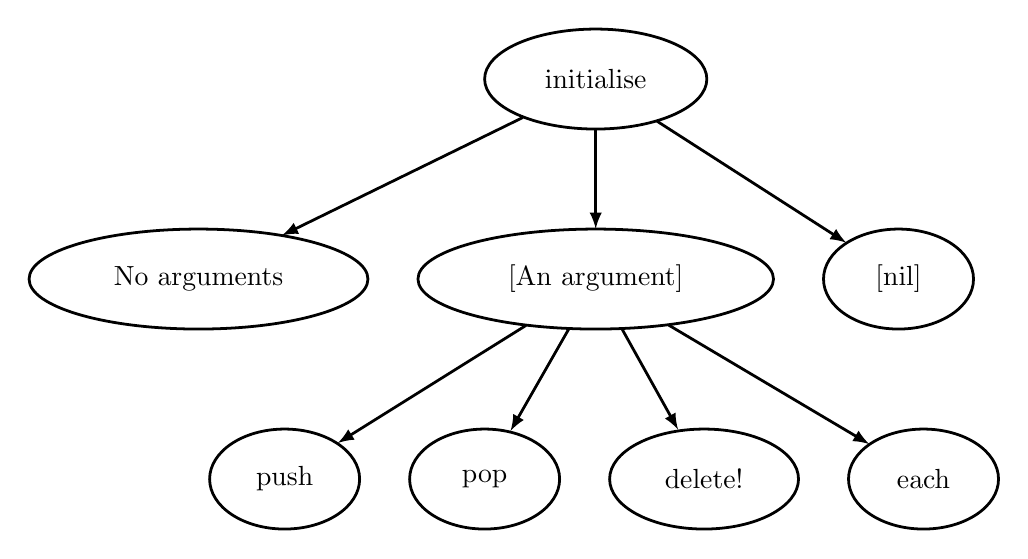
\begin{tikzpicture}[>=latex,line join=bevel,]
  \pgfsetlinewidth{1bp}
%%
\pgfsetcolor{black}
  % Edge: initialise -> a3
  \draw [->] (226.06bp,146.83bp) .. controls (243.27bp,135.78bp) and (267.27bp,120.36bp)  .. (294.24bp,103.05bp);
  % Edge: initialise -> a2
  \draw [->] (204bp,143.7bp) .. controls (204bp,135.98bp) and (204bp,126.71bp)  .. (204bp,108.1bp);
  % Edge: initialise -> a1
  \draw [->] (177.77bp,148.16bp) .. controls (156.04bp,137.52bp) and (124.82bp,122.24bp)  .. (91.021bp,105.7bp);
  % Edge: a2 -> b4
  \draw [->] (230.19bp,73.465bp) .. controls (249.06bp,62.268bp) and (274.5bp,47.175bp)  .. (302.49bp,30.576bp);
  % Edge: a2 -> b2
  \draw [->] (194.32bp,72.055bp) .. controls (189.53bp,63.679bp) and (183.66bp,53.404bp)  .. (173.32bp,35.307bp);
  % Edge: a2 -> b3
  \draw [->] (213.44bp,72.055bp) .. controls (218.04bp,63.801bp) and (223.67bp,53.701bp)  .. (233.65bp,35.789bp);
  % Edge: a2 -> b1
  \draw [->] (178.87bp,73.291bp) .. controls (161.4bp,62.375bp) and (138.11bp,47.819bp)  .. (111.13bp,30.956bp);
  % Node: b4
\begin{scope}
  \definecolor{strokecol}{rgb}{0.0,0.0,0.0};
  \pgfsetstrokecolor{strokecol}
  \draw (322bp,18bp) ellipse (27bp and 18bp);
  \draw (322bp,18bp) node {each};
\end{scope}
  % Node: a1
\begin{scope}
  \definecolor{strokecol}{rgb}{0.0,0.0,0.0};
  \pgfsetstrokecolor{strokecol}
  \draw (61bp,90bp) ellipse (61bp and 18bp);
  \draw (61bp,90bp) node {No arguments};
\end{scope}
  % Node: a3
\begin{scope}
  \definecolor{strokecol}{rgb}{0.0,0.0,0.0};
  \pgfsetstrokecolor{strokecol}
  \draw (313bp,90bp) ellipse (27bp and 18bp);
  \draw (313bp,90bp) node {[nil]};
\end{scope}
  % Node: initialise
\begin{scope}
  \definecolor{strokecol}{rgb}{0.0,0.0,0.0};
  \pgfsetstrokecolor{strokecol}
  \draw (204bp,162bp) ellipse (40bp and 18bp);
  \draw (204bp,162bp) node {initialise};
\end{scope}
  % Node: b1
\begin{scope}
  \definecolor{strokecol}{rgb}{0.0,0.0,0.0};
  \pgfsetstrokecolor{strokecol}
  \draw (92bp,18bp) ellipse (27bp and 18bp);
  \draw (92bp,18bp) node {push};
\end{scope}
  % Node: b2
\begin{scope}
  \definecolor{strokecol}{rgb}{0.0,0.0,0.0};
  \pgfsetstrokecolor{strokecol}
  \draw (164bp,18bp) ellipse (27bp and 18bp);
  \draw (164bp,18bp) node {pop};
\end{scope}
  % Node: b3
\begin{scope}
  \definecolor{strokecol}{rgb}{0.0,0.0,0.0};
  \pgfsetstrokecolor{strokecol}
  \draw (243bp,18bp) ellipse (34bp and 18bp);
  \draw (243bp,18bp) node {delete!};
\end{scope}
  % Node: a2
\begin{scope}
  \definecolor{strokecol}{rgb}{0.0,0.0,0.0};
  \pgfsetstrokecolor{strokecol}
  \draw (204bp,90bp) ellipse (64bp and 18bp);
  \draw (204bp,90bp) node {[An argument]};
\end{scope}
%
\end{tikzpicture}

